% interactcadsample.tex
% v1.03 - April 2017

\documentclass[]{interact}

\usepackage{epstopdf}% To incorporate .eps illustrations using PDFLaTeX, etc.
\usepackage{subfigure}% Support for small, `sub' figures and tables
%\usepackage[nolists,tablesfirst]{endfloat}% To `separate' figures and tables from text if required

\usepackage{natbib}% Citation support using natbib.sty
\bibpunct[, ]{(}{)}{;}{a}{}{,}% Citation support using natbib.sty
\renewcommand\bibfont{\fontsize{10}{12}\selectfont}% Bibliography support using natbib.sty

\theoremstyle{plain}% Theorem-like structures provided by amsthm.sty
\newtheorem{theorem}{Theorem}[section]
\newtheorem{lemma}[theorem]{Lemma}
\newtheorem{corollary}[theorem]{Corollary}
\newtheorem{proposition}[theorem]{Proposition}

\theoremstyle{definition}
\newtheorem{definition}[theorem]{Definition}
\newtheorem{example}[theorem]{Example}

\theoremstyle{remark}
\newtheorem{remark}{Remark}
\newtheorem{notation}{Notation}


% tightlist command for lists without linebreak
\providecommand{\tightlist}{%
  \setlength{\itemsep}{0pt}\setlength{\parskip}{0pt}}



\usepackage{hyperref}
\usepackage[utf8]{inputenc}
\def\tightlist{}


\begin{document}


\articletype{ORIGINAL RESEARCH ARTICLE}

\title{Size matters: Divergent morphology in elliptical bifaces from
sites in the American Southeast articulates with distinct local
reduction practices}


\author{\name{Robert Z. Selden, Jr.$^{a}$, John E. Dockall$^{b}$, and
David H. Dye$^{c}$}
\affil{$^{a}$Heritage Research Center, Stephen F. Austin State
University; Department of Biology, Stephen F. Austin State University;
Texas Archeological Research Laboratory, The University of Texas at
Austin; and Cultural Heritage Department, Jean Monnet
University; $^{b}$Stantec, Inc.; $^{c}$Department of Earth Sciences, The
University of Memphis}
}

\thanks{CONTACT Robert Z. Selden,
Jr.. Email: \href{mailto:zselden@sfasu.edu}{\nolinkurl{zselden@sfasu.edu}}, John
E.
Dockall. Email: \href{mailto:john.dockall@stantec.com}{\nolinkurl{john.dockall@stantec.com}}, and
David H.
Dye. Email: \href{mailto:daviddye@memphis.edu}{\nolinkurl{daviddye@memphis.edu}}}

\maketitle

\begin{abstract}
Elliptical bifaces are prevalent at Mississipian sites throughout the
American Southeast. Those from Millsap Cache and Jowell Farm comprise
two of the largest samples of this ill-understood stone tool from the
ancestral Caddo area. Bifaces from Millsap Cache were reportedly
produced using Kay County flint, while those from Jowell Farm were
manufactured using Edwards chert, providing for an empirical test of
morphological differences as a function of raw material. The sample of
elliptical bifaces was divided into two size classes; one conceptually
reflective of production (large), and the other with local reduction
practices (small). Size classes were used to assess whether
modifications by Caddo knappers may have yielded
similar---convergent---biface shape in the small class. Size classes
were also used to test the hypothesis that greater morphological
variation would be apparent in the small class due to idiosyncratic
responses related to local retouch practices. Results demonstrate that
elliptical biface shape does not differ by raw material, but size does,
suggesting that a shared and morphologically-consistent mental template
was maintained independent of biface size. The subsequent analysis of
elliptical biface morphology by size class demonstrated that size does
not differ by raw material in the large class, but in the small class,
it does. This finding supports the argument that elliptical biface
morphology diverges through local reduction practices. As expected,
greater shape diversity occurs in the small class, where Jowell Farm
bifaces were found to be more morphologically diverse than those from
Millsap Cache. Distinct local reduction practices are advanced as the
driver of extant morphological differences found in elliptical bifaces.
\end{abstract}

\begin{keywords}
American Southeast; Caddo; NAGPRA; archaeology; ovoid biface; Jowell
knife; Jowell knives; Jowell biface; lithics; parallel oblique flaking;
archaeoinformatics; museum studies; digital humanities; non-Western art
history; geometric morphometrics; STEM; STEAM
\end{keywords}

\begin{quote}
\textit{This process of comparison, of recognising in one form a definite permutation or deformation of another, apart altogether from a precise and adequate understanding of the original 'type' or standard of comparison, lies within the immediate province of mathematics, and finds its solution in the elementary use of a certain method of the mathematician} \citep{RN7522}.
\end{quote}

\hypertarget{introduction}{%
\section{Introduction}\label{introduction}}

Elliptical bifaces have a deep history in eastern North America
extending from the Middle Archaic to well past European contact. In many
instances they have been deposited in caches, which may represent large,
corporate bundles decommissioned amid polity demise or radical
transformations in social practice. Stylistic changes are evident in
both length and width for these bifaces, and result in great variability
in shape and size. While some undoubtedly were knapped for every-day,
mundane uses, others were crafted from exotic cherts and reflect
non-utilitarian uses. The \emph{oversize} or \emph{exaggerated} forms,
mimicking combat weapons, are often referred to as symbolic weaponry.
Such objects are typically those ``whose size, delicacy, material of
manufacture, and craftsmanship are outside the bounds of any weapon that
might have been actually used'' \citep[624]{RN11177}.

The earliest elliptical bifaces, associated with Middle Archaic period,
recovered as Benton caches (4500---4000 BCE) in the Mid-South
\citep{RN11179}, are clearly non-utilitarian, as they ``meet the
expectations of sacred markers for secular exchange''
\citep[143]{RN11178}. In the western Middle Tennessee Valley, the
Pickwick Burial Complex \citep[94]{RN11180}, dating to the Late
Archaic/Gulf Formational period (3000---300 BCE) exhibits a continuation
of bipointed blades, some notched or truncated, found in ritual caches
and ceremonially broken. Elliptical bifaces find their most dramatic
expression as Caddoan and Mississippian exaggerated, symbolic weaponry.
Mississippian Ramey knives, dating from c.~CE 1000 to 1300 are found
associated with Cahokia political dynamics. The slightly later Duck
River sword-form bifaces (CE 1275-1400) continue the emphasis on
high-quality knapping and long-distance circulation. Such lanceolate
blades, although smaller, continue into the early seventeenth century
when they serve as regalia among political and social elites in ritual
performances.

\begin{figure}\centering
\includegraphics[width=0.9\linewidth]{figs/map.png}
\caption{Location of Millsap Cache, Jowell Farm, and other sites mentioned in the text. Elliptical bifaces have been found in every major drainage basin in the ancestral Caddo area (white).}
\label{fig:map}
\end{figure}

\hypertarget{parallel-oblique-flaking}{%
\subsection{Parallel-oblique flaking}\label{parallel-oblique-flaking}}

When compared with other large finished bifaces in the region, the
distinctive parallel oblique flake scar patterns on both faces of the
elliptical bifaces for all, or virtually all, of their length is unique
(Figure \ref{fig:illustration}). The absence of identified preforms for
this artifact type makes technological and/or attribute-based
discriminations related to manufacture a challenge; however, one
potential preform was recovered from mortuary contexts at Belcher Mound
(Figure \ref{fig:illustration}c). The projection of ritual and/or
symbolic interpretation/s that articulate with this flake scar pattern
is not possible at this time. Parallel oblique flake scar patterns are
known to be characteristic of Guerrero arrow points found at missions in
Texas \citep{RN9610}, several dart point types of the late Paleoindian
period \citep{RN8584,RN7935,RN11182, RN9843,RN8143,RN10117,RN11181}, and
this distinctive flaking pattern has also been inferred from ceramic
motifs in Peru \citep{RN7938}.

Parallel oblique flake scar patterns are not characteristic of any of
the larger bifaces and bifacial knives in the American Southeast; thus,
technological, cultural, or symbolic relationships between the
elliptical bifaces and Guerrero arrow points or Angostura dart points
are not suggested here. The technological choice to use parallel oblique
flaking in finishing these elliptical bifaces most likely represents, at
minimum, a stylistic choice by knappers limited to this specific
implement; although, that may have been a functionally-relevant choice
given their shape and size. In some respects, the decision to employ
parallel oblique flaking is as distinctive as the presence---although
not diagnostic \citep{RN6170}---of the flat and expanding flake scar
pattern observed on Gahagan and Copena bifaces.

\begin{figure}\centering
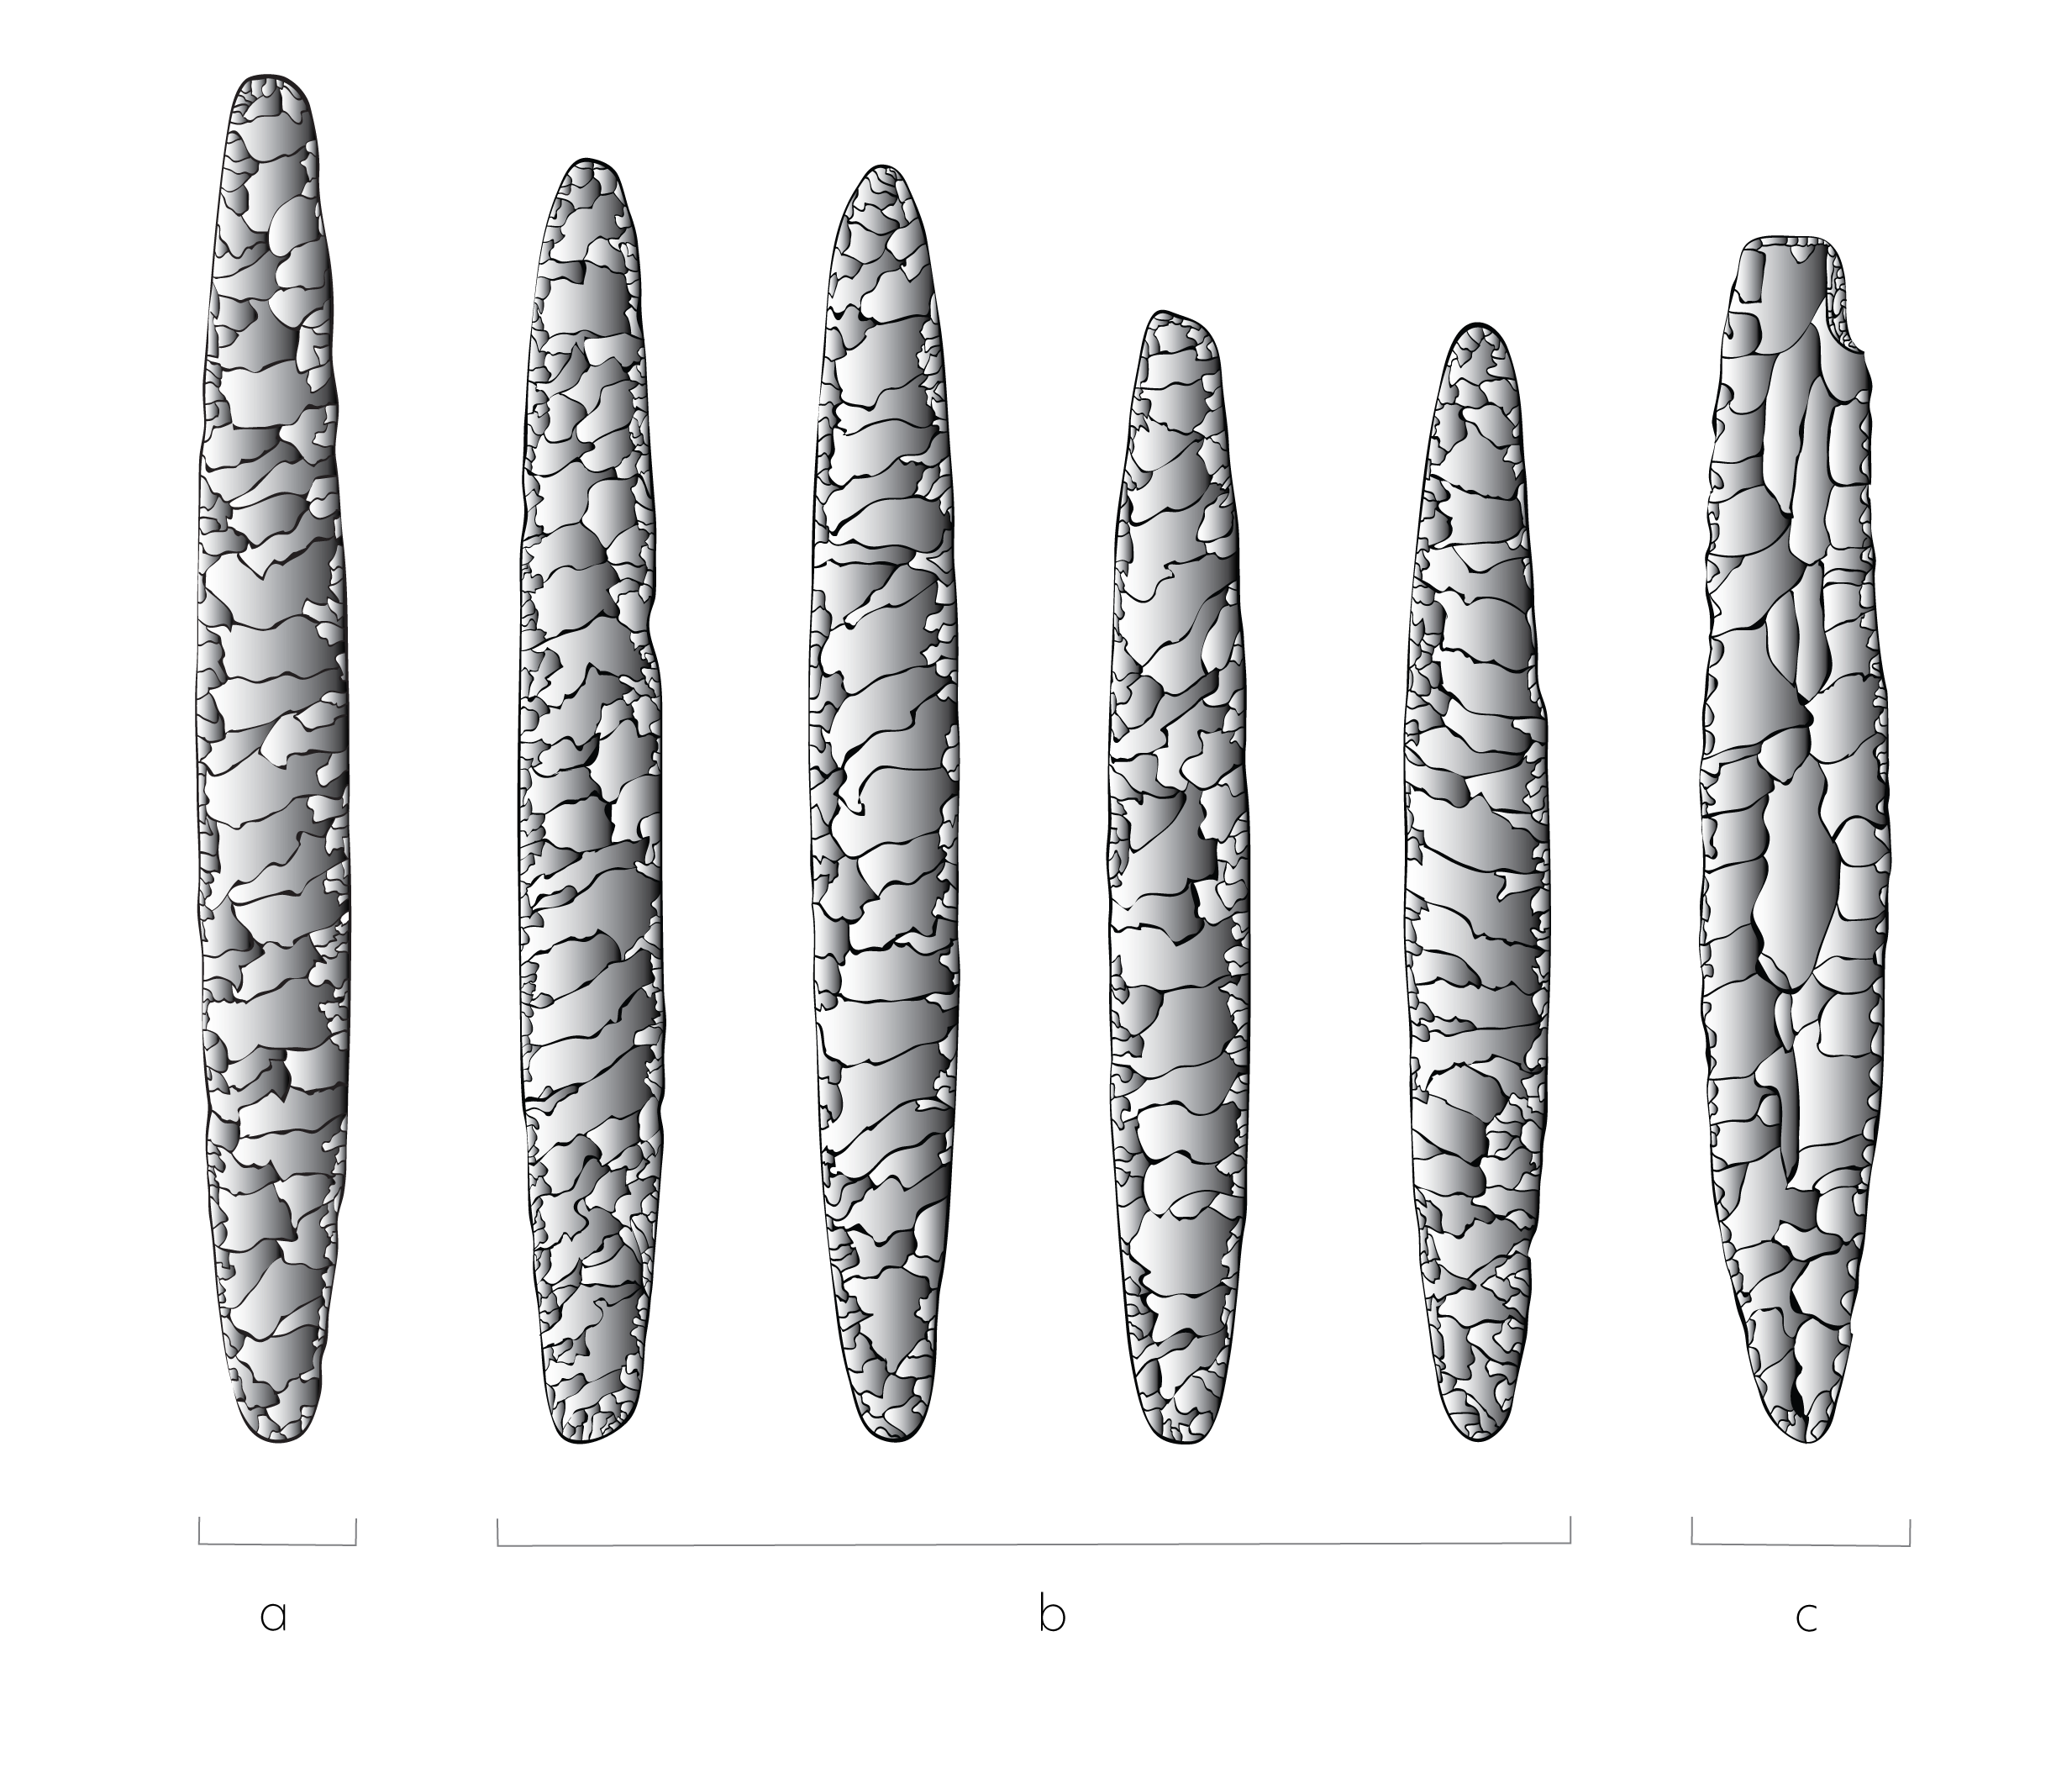
\includegraphics[width=0.9\linewidth]{figs/elliptical.illustration.png}
\caption{Illustrated elliptical bifaces from a, an unknown location; b, Jowell Farm; and c, Belcher Mound highlighting parallel oblique flaking used in production. The specimen from Belcher Mound is a potential preform exhibiting parallel oblique removals consistent with elliptical bifaces from other sites in the region.}
\label{fig:illustration}
\end{figure}

\hypertarget{methods-and-results}{%
\section{Methods and results}\label{methods-and-results}}

To assess the variable impacts that Caddo retouch practices may have had
on general morphology, the sample of elliptical bifaces was binned into
two size classes using centroid size
(\href{https://seldenlab.github.io/elliptical.bifaces/}{Supplementary
Materials}). Due to potential morphological differences associated with
the use of two distinct raw materials (Kay County flint and Edwards
chert), the sample was subset by site prior to calculating the mean
centroid size for each. Raw material for bifaces from Millsap Cache were
identified by \citet{RN11461} as Kay County flint, and those from Jowell
Farm were identified as Edwards Chert due to their size, the colours
that they fluoresce beneath low and high frequency UV light, and the
paucity of similarly large locally-available raw material sources.
Bifaces larger than the mean were assigned to the large category, those
smaller than the mean were assigned to the small category, and the two
datasets were joined in advance of analysis
(\href{https://seldenlab.github.io/elliptical.bifaces/}{Supplementary
Materials}).

Elliptical bifaces from Millsap Cache and Jowell Farm were used to
examine whether biface morphology remains stable or expresses
morphological variability by site/raw material
(\href{https://seldenlab.github.io/elliptical.bifaces/gm---siteraw-material.html}{Supplementary
Materials}). Prior to landmarking, elliptical bifaces were oriented with
the most heavily retouched edge at top right (Figure
\ref{fig:elliptical}). Some bifaces include multiple areas of heavy
retouch at the top and bottom of the same lateral edge (Figure
\ref{fig:elliptical}:b, c, d, and e), while others (Figure
\ref{fig:elliptical}:f) include one retouched edge at top right and
another at bottom left.

\begin{figure}\centering
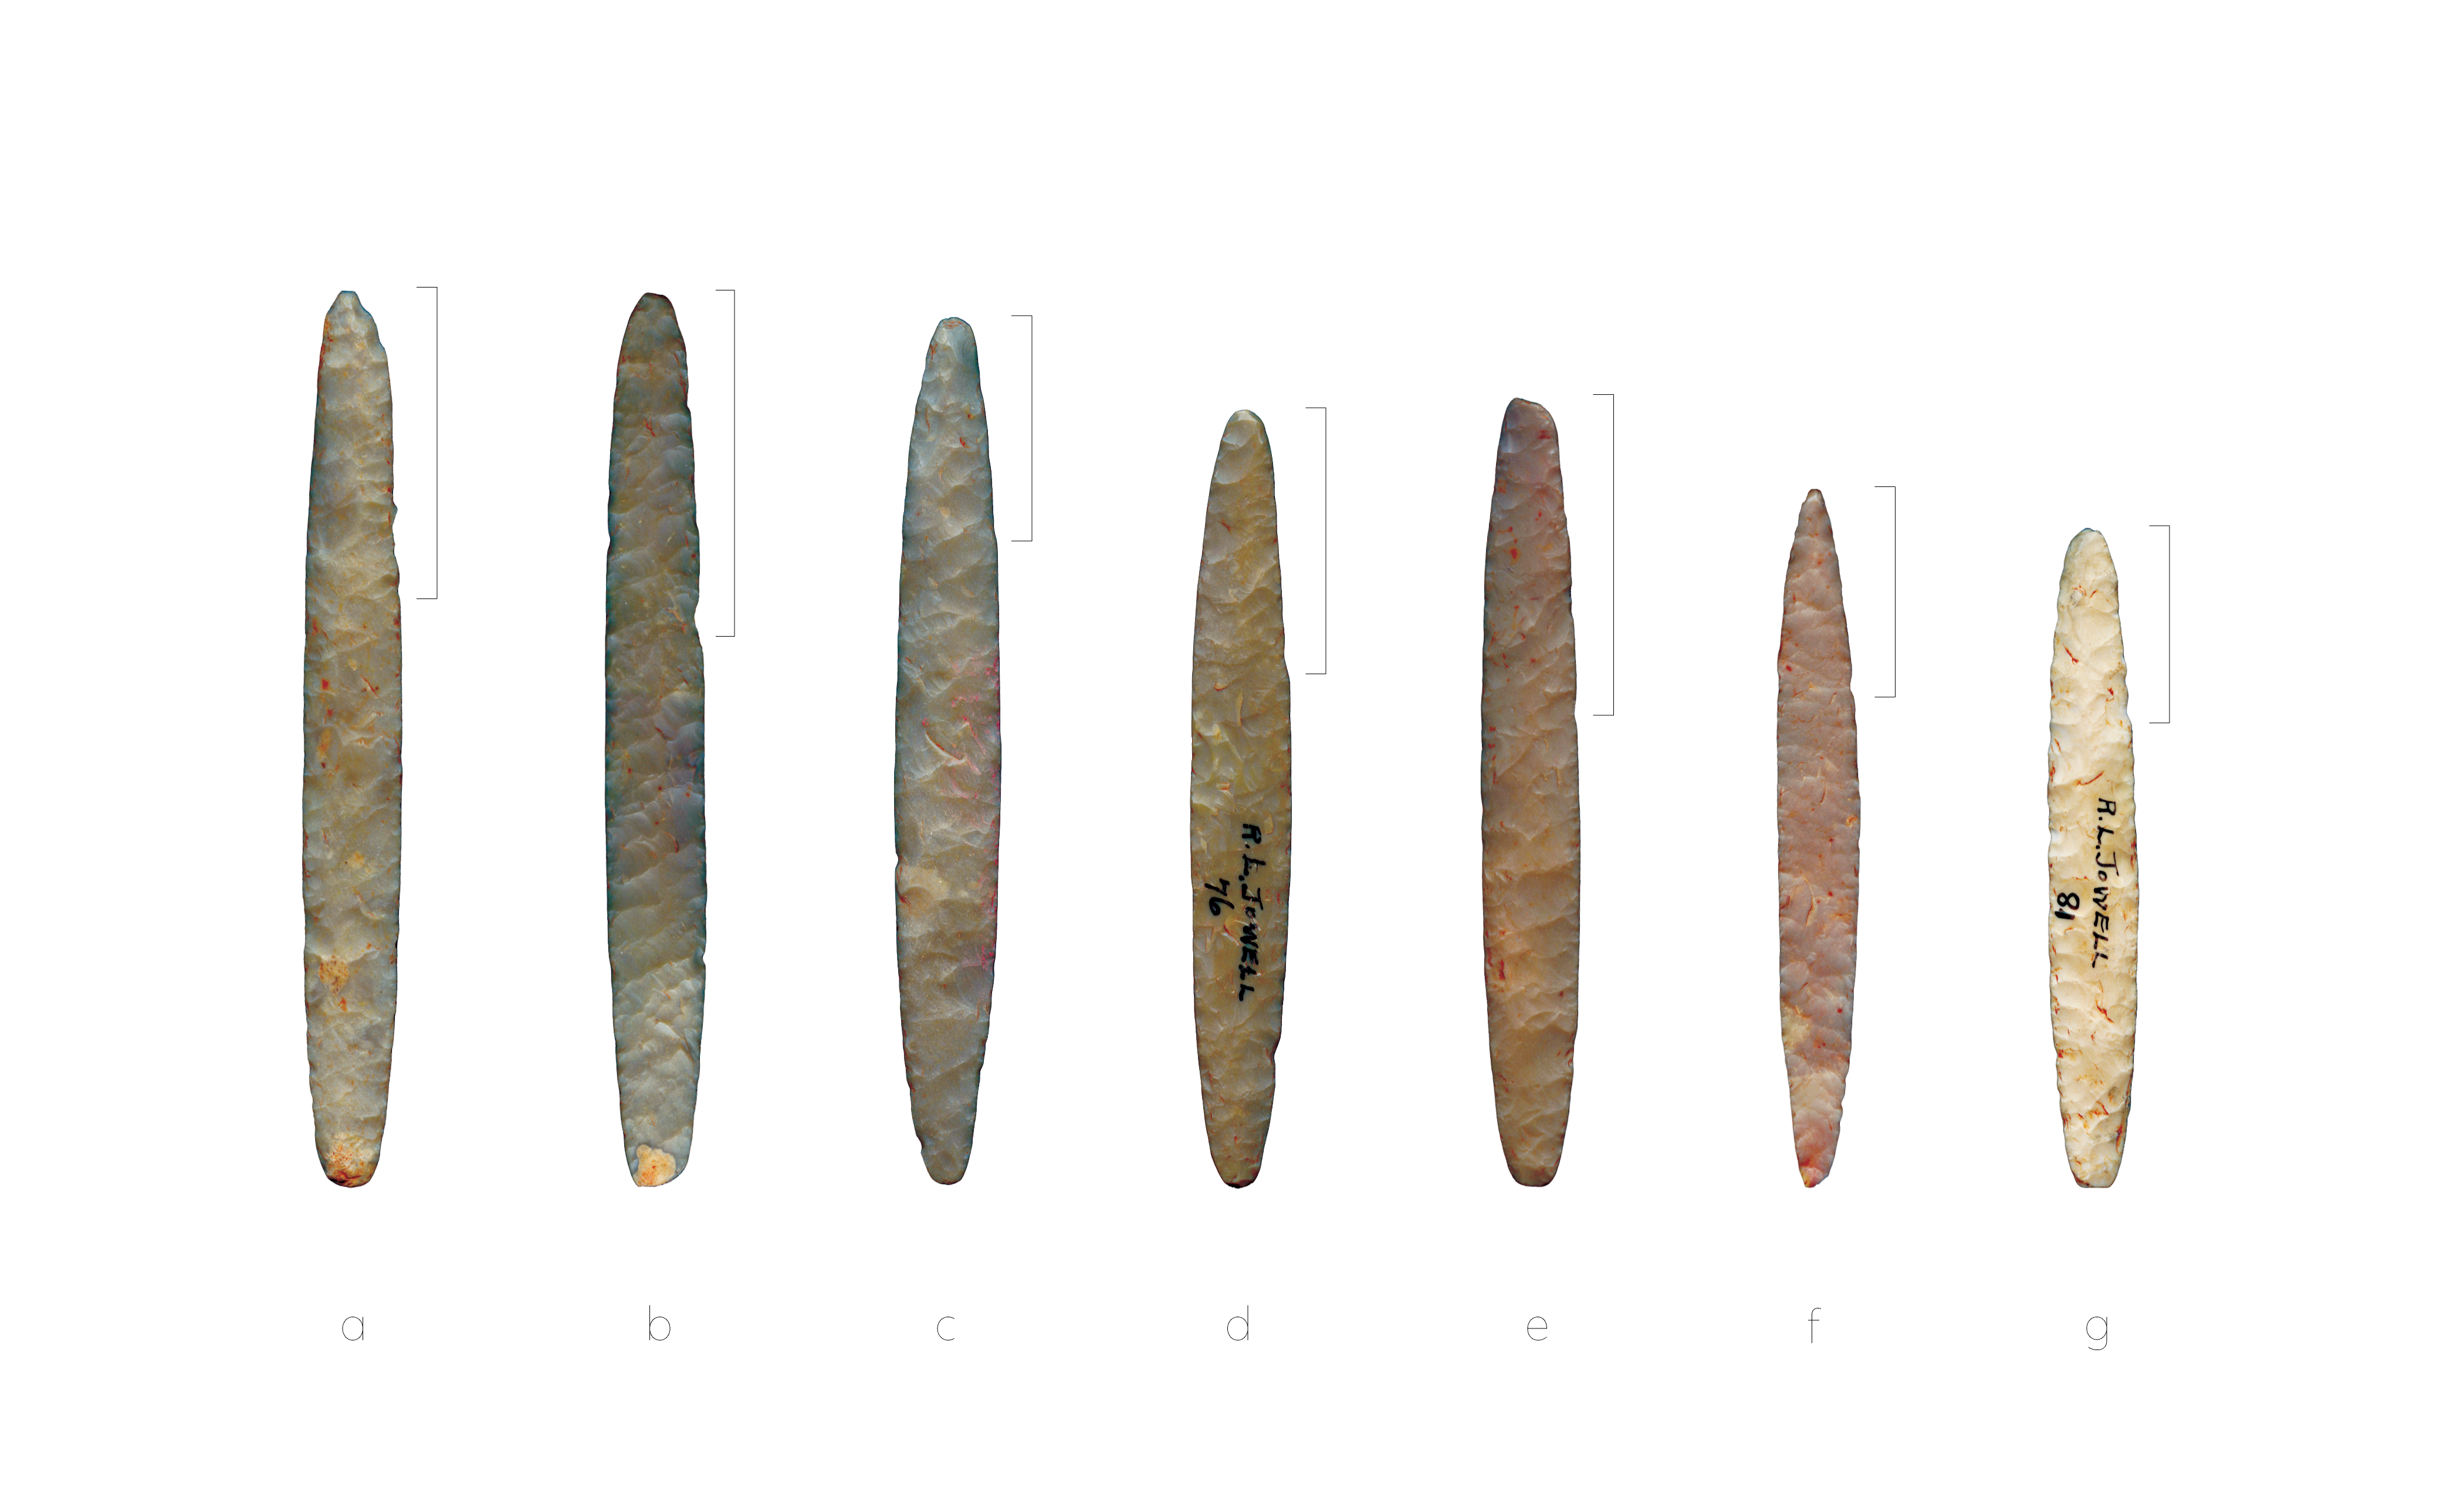
\includegraphics[width=\linewidth]{figs/ellipticalbifaces.png}
\caption{Selected elliptical bifaces from the Jowell Farm site highlighting the most heavily retouched area at top right identified using a modified version of the flaking index developed by \citet{RN11099}.}
\label{fig:elliptical}
\end{figure}

To identify which edge was most heavily retouched, we employed a
modified approach to the flaking index developed by \citet{RN11099}. The
modified approach uses counts of flake scars from both sides of each
edge in the two most heavily worked areas, paired with a measure of edge
length inclusive of curvature, which was calculated using ImageJ
\citep{RN11146,RN11147,RN11148}. The number of flake scars was
subsequently divided by the length of the worked edge, with the most
heavily worked edge identified by the greater value.

\hypertarget{geometric-morphometrics}{%
\subsection{Geometric morphometrics}\label{geometric-morphometrics}}

The same landmark/semilandmark configuration was used for both analyses,
and the landmarking protocol employs three landmarks; two horizontal
tangents (top/bottom), and the third placed at the furthest extent of
the retouched edge bearing the heaviest amount of retouch (see Figure
\ref{fig:elliptical}). Equidistant semilandmarks were placed between
each landmark, applied using R \citep{R} and the \texttt{StereoMorph}
package \citep{RN9091}.

\hypertarget{generalised-procrustes-analysis}{%
\subsubsection{Generalised Procrustes
Analysis}\label{generalised-procrustes-analysis}}

Landmark data were aligned to a global coordinate system
\citep{RN8477,RN7502,RN11622,RN11623,RN11563}, achieved through
generalised Procrustes superimposition \citep{RN11138,RN478,RN1646} in R
using the \texttt{geomorph} and \texttt{RRPP} packages
\citep{RN1655,RN11775,RN11530,RN1774,RN8605}. Procrustes superimposition
translates and rotates the coordinate data to allow for comparisons
among objects, while also scaling each biface using unit-centroid
size---the square root of the sum of squared distances from each
landmark to the specimen's centroid
\citep{RN11139,RN11140,RN11564,RN478}. The \texttt{geomorph} package
uses a partial Procrustes superimposition that projects the aligned
specimens into tangent space subsequent to alignment in preparation for
the use of multivariate methods that assume linear space (Figure
\ref{fig:gpa}) \citep{RN11141,RN11142,RN1646,RN11563}.

\begin{figure}\centering
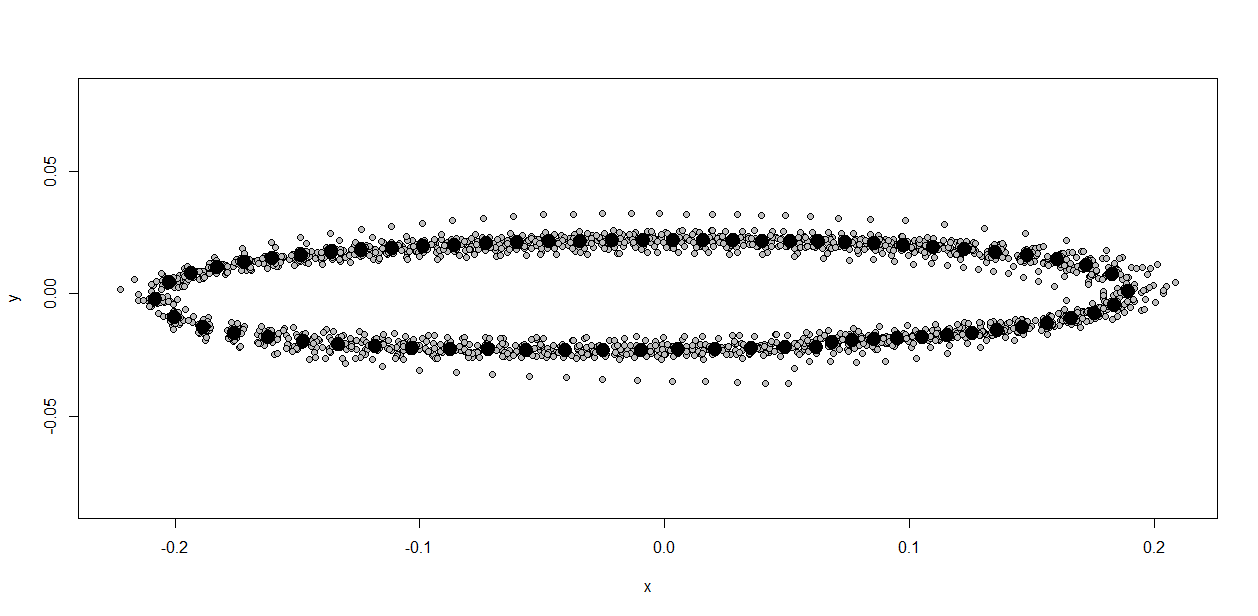
\includegraphics[width=\linewidth]{figs/gpa.png}
\caption{Results of generalised Procrustes analysis for elliptical bifaces from the Millsap Cache and Jowell Farm. Mean consensus configuration shown in black; individual bifaces in gray.}
\label{fig:gpa}
\end{figure}

\hypertarget{principal-components-analysis}{%
\subsubsection{Principal Components
Analysis}\label{principal-components-analysis}}

Principal components analysis \citep{RN1746} was used to visualise shape
variation among the elliptical bifaces, and the scatterplot and convex
hulls represent the dispersion of shapes in tangent space (Figure
\ref{fig:pca}) \citep{RN8633,RN5616,RN11143,RN7550}. Shape space
described by each principal axis is commonly visualized using thin-plate
spline warping of a reference image or 3D mesh \citep{RN1731,RN479}.

\begin{figure}\centering
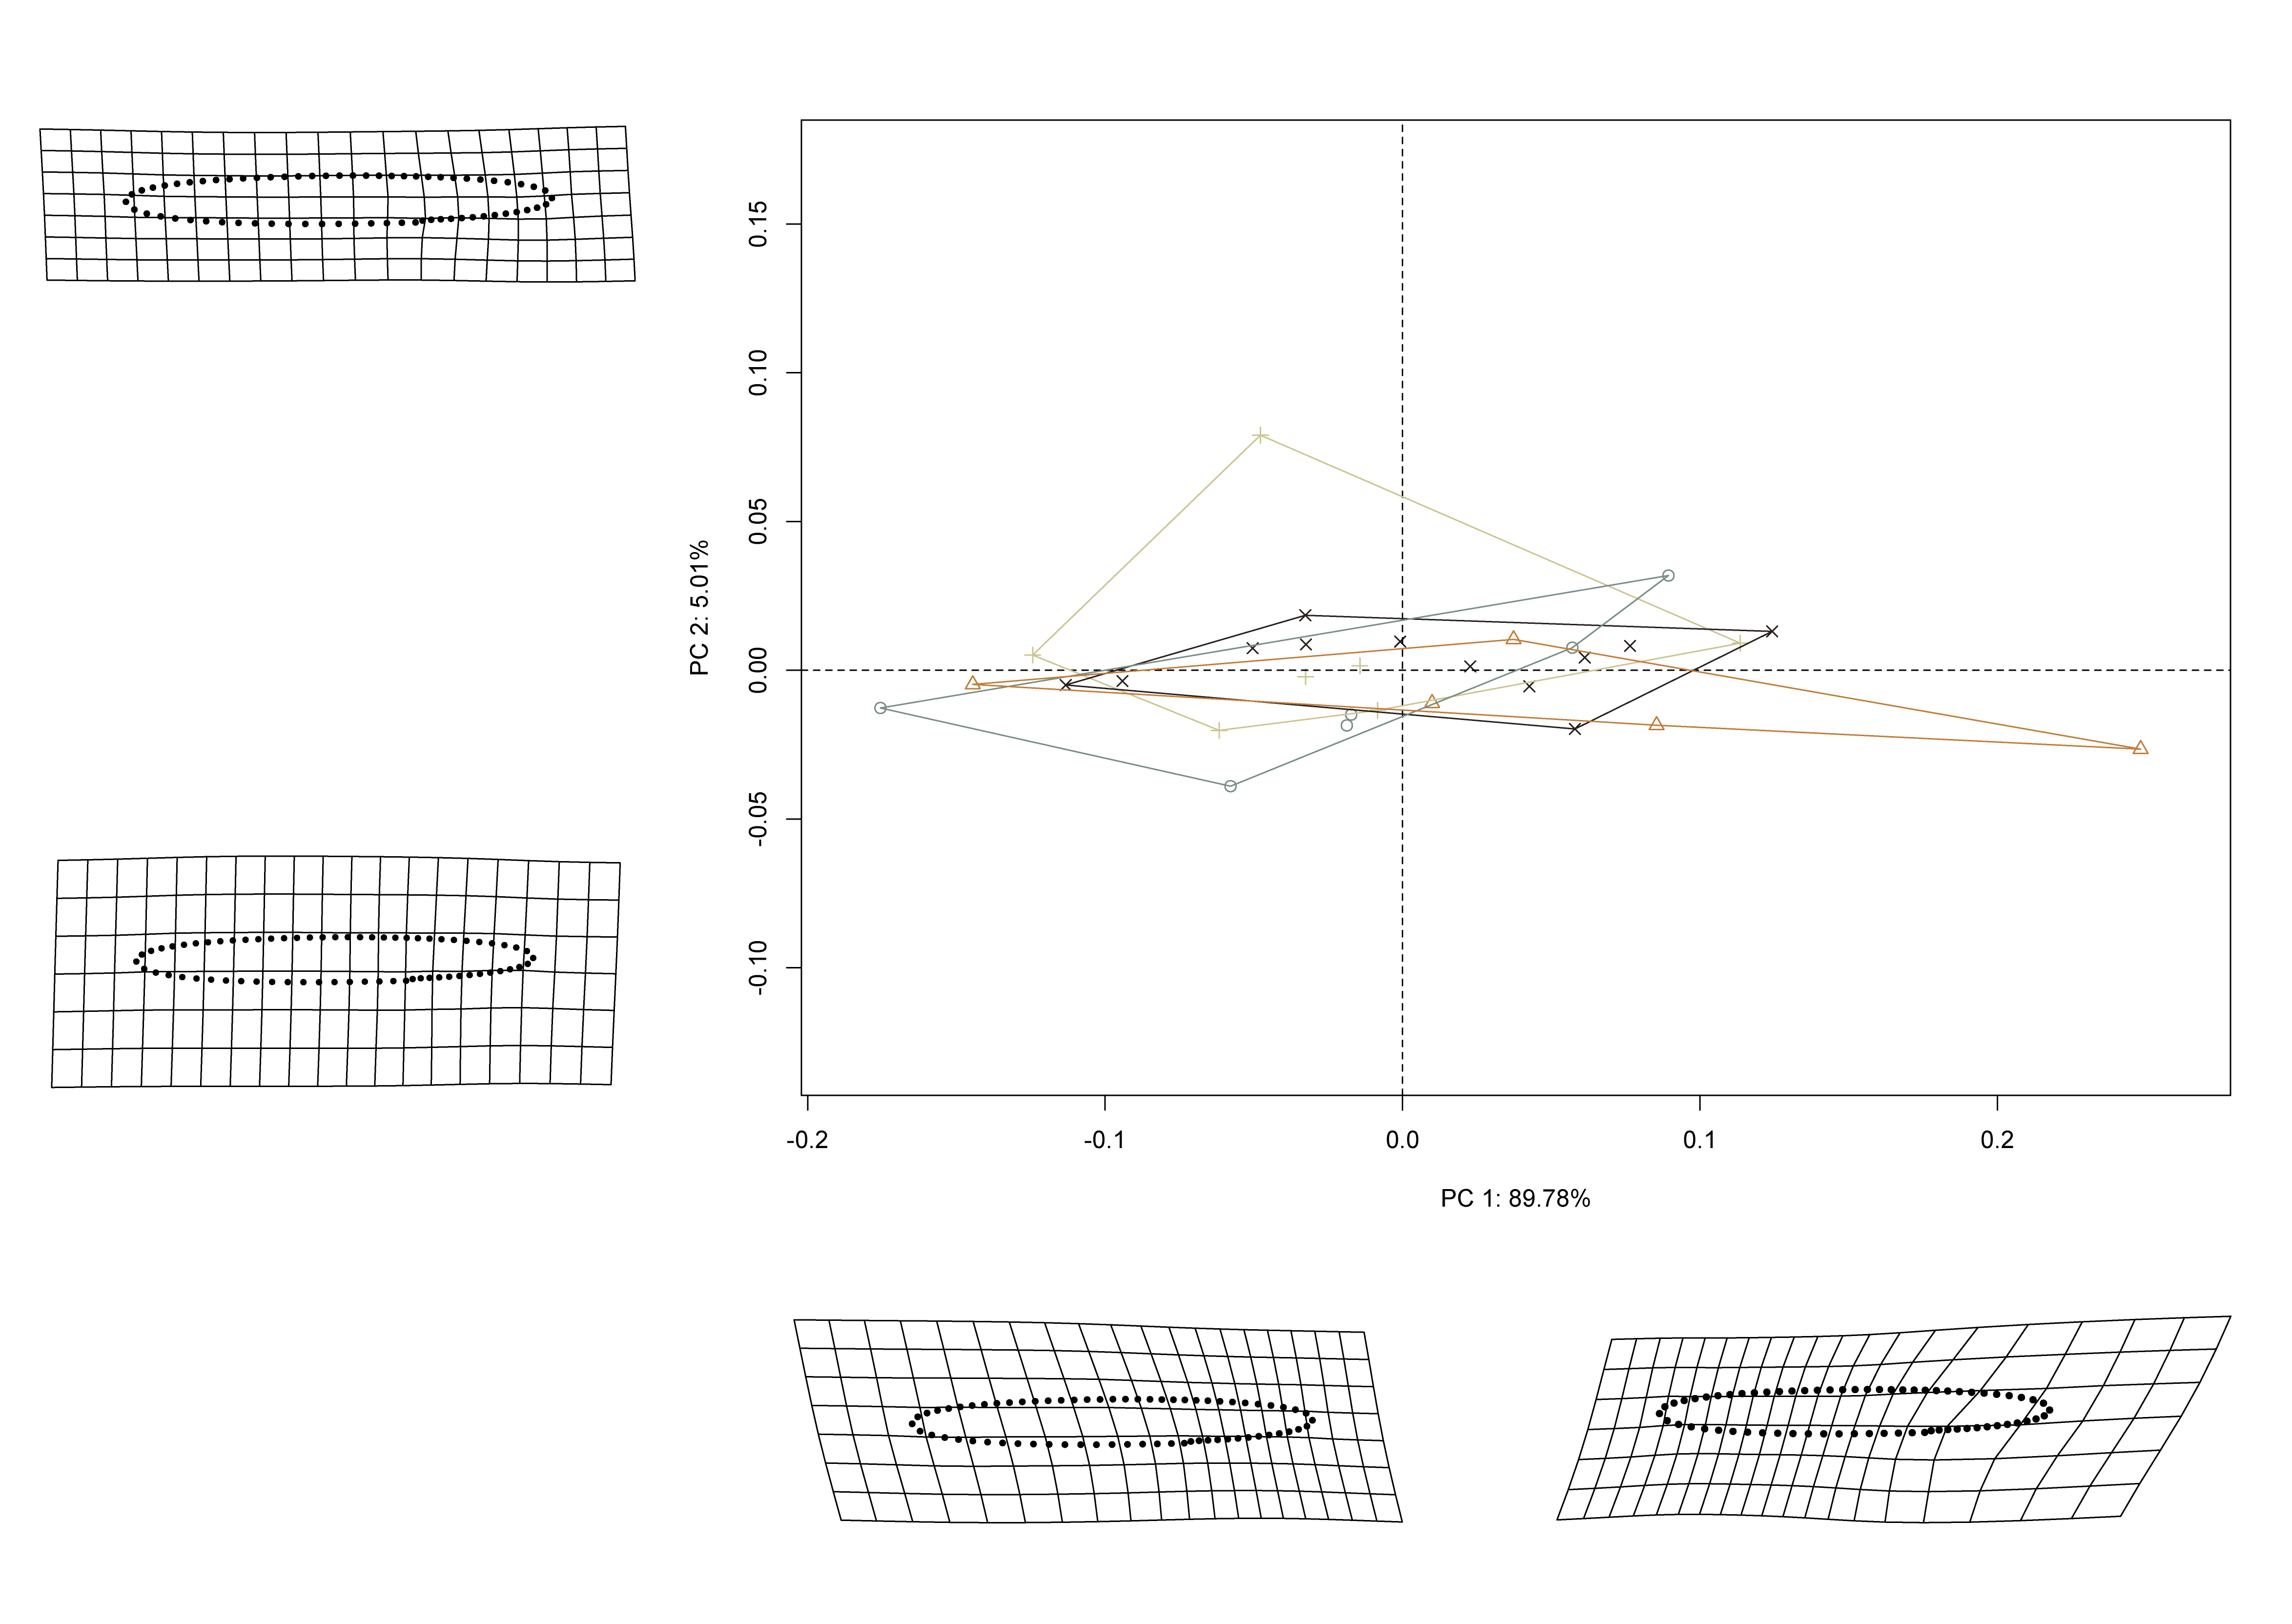
\includegraphics[width=\linewidth]{figs/pca.png}
\caption{PCA summarizing shape variation in elliptical bifaces by site and size class. }
\label{fig:pca}
\end{figure}

\hypertarget{procrustes-anova}{%
\subsubsection{Procrustes ANOVA}\label{procrustes-anova}}

To assess whether shape changed with size (allometry), and whether shape
and size differed by raw material and size class, Procrustes ANOVAs
\citep{RN1749} were run that enlist effect-sizes (zscores) computed as
standard deviates of the generated sampling distributions
\citep{RN1756}. A residual randomization permutation procedure (RRPP; n
= 10,000 permutations) was used for all Procrustes ANOVAs
\citep{RN1655,RN11775}, which has higher statistical power and a greater
ability to identify patterns in the data should they be present
\citep{RN1719}.

The test for allometry did not return a significant result, suggesting
that elliptical biface shape and size may follow a pattern of isometry,
where shape remains constant throughout the reduction/retouch process
(\href{https://seldenlab.github.io/elliptical.bifaces/}{Supplementary
Materials}). Elliptical bifaces were morphologically consistent in shape
across all analyses
(\href{https://seldenlab.github.io/elliptical.bifaces/}{Supplementary
Materials}). Results demonstrated a significant difference in size by
site/raw material (RRPP = 10,000, Pr(\textgreater F) = 0.0007); however,
the subsequent analysis by size class demonstrated that the pattern is
more readily attributable to reduction practices/intensity rather than
nodule and raw material size
(\href{https://seldenlab.github.io/elliptical.bifaces/}{Supplementary
Materials}).

The analysis of morphology by size class demonstrated a significant
difference in size between size classes (expected); however, the pattern
deviated from our expectations. Elliptical bifaces from Jowell Farm
differ in neither shape nor size between size classes
(\href{https://seldenlab.github.io/elliptical.bifaces/}{Supplementary
Materials}). Elliptical bifaces in the large and small size classes from
Millsap Cache differ significantly in size (RRPP = 10,000,
Pr\textgreater d = 0.0035), but not shape
(\href{https://seldenlab.github.io/elliptical.bifaces/}{Supplementary
Materials}). Pairwise comparisons demonstrate that elliptical bifaces
from Millsap Cache and Jowell Farm in the large size class are
morphologically consistent, but those in the small size class differ in
size (RRPP = 10,000, Pr\textgreater d = 0.0001)
(\href{https://seldenlab.github.io/elliptical.bifaces/}{Supplementary
Materials}).

Thus, the pattern that emerges is one of differential retouch
\emph{intensity}, where isometric retouch strategies of Caddo knappers
at Millsap Cache articulate with a different reduction practice thought
to be associated with locally abundant raw material (Kay County flint).
This finding is contrasted with the comparatively minimal retouch
intensity of another group (Jowell Farm) where local raw materials were
of poor quality and insufficient size, yielding a situation where it was
necessary to import raw material from an extralocal source (Edwards
chert).

\hypertarget{morphological-disparity}{%
\subsubsection{Morphological disparity}\label{morphological-disparity}}

An analysis of morphological disparity was used to identify potential
differences in morphological diversity between size classes
\citep{RN11107,RN7041,RN5694}. No difference was found in elliptical
biface shape or size by site/raw material, but the comparison of
morphological diversity by size class demonstrated that biface shapes in
the small size class from Jowell Farm occupy a significantly greater
range of morphospace than those from Millsap Cache.

The comparison of morphological disparity by size class demonstrated
that elliptical biface shapes in the small size class at Jowell Farm
occupy a significantly greater range of morphospace than those from
Millsap Cache. This pattern suggests that the comparatively minimal
retouch intensity associated with Caddo knappers at Jowell Farm may have
been more targeted---potentially due to a lack of abundant local raw
material of sufficient quality and size---resulting in a broader range
of biface shapes in the small size class. Conversely, results also
suggest that Caddo knappers at Millsap Cache employed a more
standardized (specialized?) approach to reduction.

\hypertarget{discussion}{%
\section{Discussion}\label{discussion}}

\hypertarget{conclusion}{%
\section{Conclusion}\label{conclusion}}

\hypertarget{acknowledgements}{%
\section*{Acknowledgement(s)}\label{acknowledgements}}
\addcontentsline{toc}{section}{Acknowledgement(s)}

Our thanks to the Caddo Nation of Oklahoma, the Caddo Nation Tribal
Council, Tribal Chairman, and Tribal Historic Preservation Office for
permission and access to NAGPRA and previously repatriated collections.
Our gratitude is also extended to Marybeth Tomka and Lauren Bussiere at
the Texas Archeological Research Laboratory for their assistance with
access to the bifaces and associated records, to Sergio Ayala and the
Gault School of Archaeological Research for access to the UV light, to
Scott Hammerstedt and Debra K. Green at the Oklahoma Archeological
Survey for their assistance with records requests, and to Marc Lavine
and Susie Fishman-Armstrong at the Sam Noble Oklahoma Museum of Natural
History for providing digital images from their collections. Thanks also
to John Harman for access to the DStretch plugin for ImageJ, which was
useful in the analysis of flake scars, and to Harry J. Shafer, Hiram F.
(Pete) Gregory, Christian S. Hoggard, and David K. Thulman for their
comments and constructive criticisms on the ongoing analyses of Caddo
biface morphology, as well as Emma Sherratt, Kersten Bergstrom, Lauren
Butaric, Dean C. Adams, and Michael L. Collyer for their constructive
criticisms, general comments, and suggestions throughout the development
of this research program.

\hypertarget{funding}{%
\section*{Funding}\label{funding}}
\addcontentsline{toc}{section}{Funding}

Components of this analytical work flow were developed and funded by a
Preservation Technology and Training grant (P14AP00138) to RZS from the
National Center for Preservation Technology and Training (NCPTT), and
additional grants to RZS from the Caddo Nation of Oklahoma, National
Forests and Grasslands in Texas (15-PA-11081300-033) and the United
States Forest Service (20-PA-11081300-074). Funding to analyse the
bifaces from Millsap Cache and Jowell Farm was provided by the Heritage
Research Center at Stephen F. Austin State University.

\hypertarget{data-management}{%
\section{Data management}\label{data-management}}

Reproducibility---the ability to recompute results---and
replicability---the chances other experimenters will achieve a
consistent result---are two foundational characteristics of successful
scientific research (Leek and Peng 2015). The analysis code associated
with this project can be accessed through the
\href{https://seldenlab.github.io/elliptical.bifaces/}{Supplementary
Materials}, is available through the GitHub repository
\url{https://github.com/seldenlab/elliptical.bifaces}, and digitally
curated on the Open Science Framework \href{https://osf.io/ph25w/}{DOI
10.17605/OSF.IO/PH25W}. The reproducible nature of this enterprise
provides a means for others to critically assess and evaluate the
various analytical components \citep{RN7434,RN7435,RN7427}, which is a
necessary requirement for the production of reliable knowledge.

Reproducibility projects in psychology and cancer biology are impacting
current research practices across all domains. Examples of reproducible
research are becoming more abundant in archaeology
\citep{RN9022,RN7818,RN10578,RN10576,RN8510,RN11097}, and the next
generation of archaeologists are learning those tools and methods needed
to reproduce and/or replicate research results \citep{RN10579}.
Reproducible and replicable research work flows are often employed at
the highest levels of humanities-based inquiries to mitigate concern or
doubt regarding proper execution, and is of particular import should the
results have---explicitly or implicitly---a major impact on scientific
progress \citep{RN10580}.

\bibliographystyle{tfcad}
\bibliography{interactcadsample.bib}


\input{"appendix.tex"}



\end{document}
